\section{Messdaten}
\label{sec:Messdaten}

Für die Durchführung der Experimente wurden zwei Zylinder mit gleicher Höhe $h=50~\si{\milli\metre}$, aber unterschiedlicher Grundfläche, als Spulenkörper verwendet. Die Grundfläche der einen Spule ($SP_K$) entspricht einem Kreis mit Radius $r=10~\si{\milli\metre}$, die der zweiten Spule einem Quadrat ($SP_Q$) mit Seitenlänge $s=20~\si{\milli\metre}$. Die Experimente werden in \autoref{sec:Auswertung} näher ausgeführt. Zur beispielhaften Darstellung der Rohdaten ist in \autoref{fig:rohdaten_abriss} der, absichtlich herbeigeführte, Abriss des Drahtes während einer Wickeloperation dargestellt.

\begin{figure}[H]
    \centering
    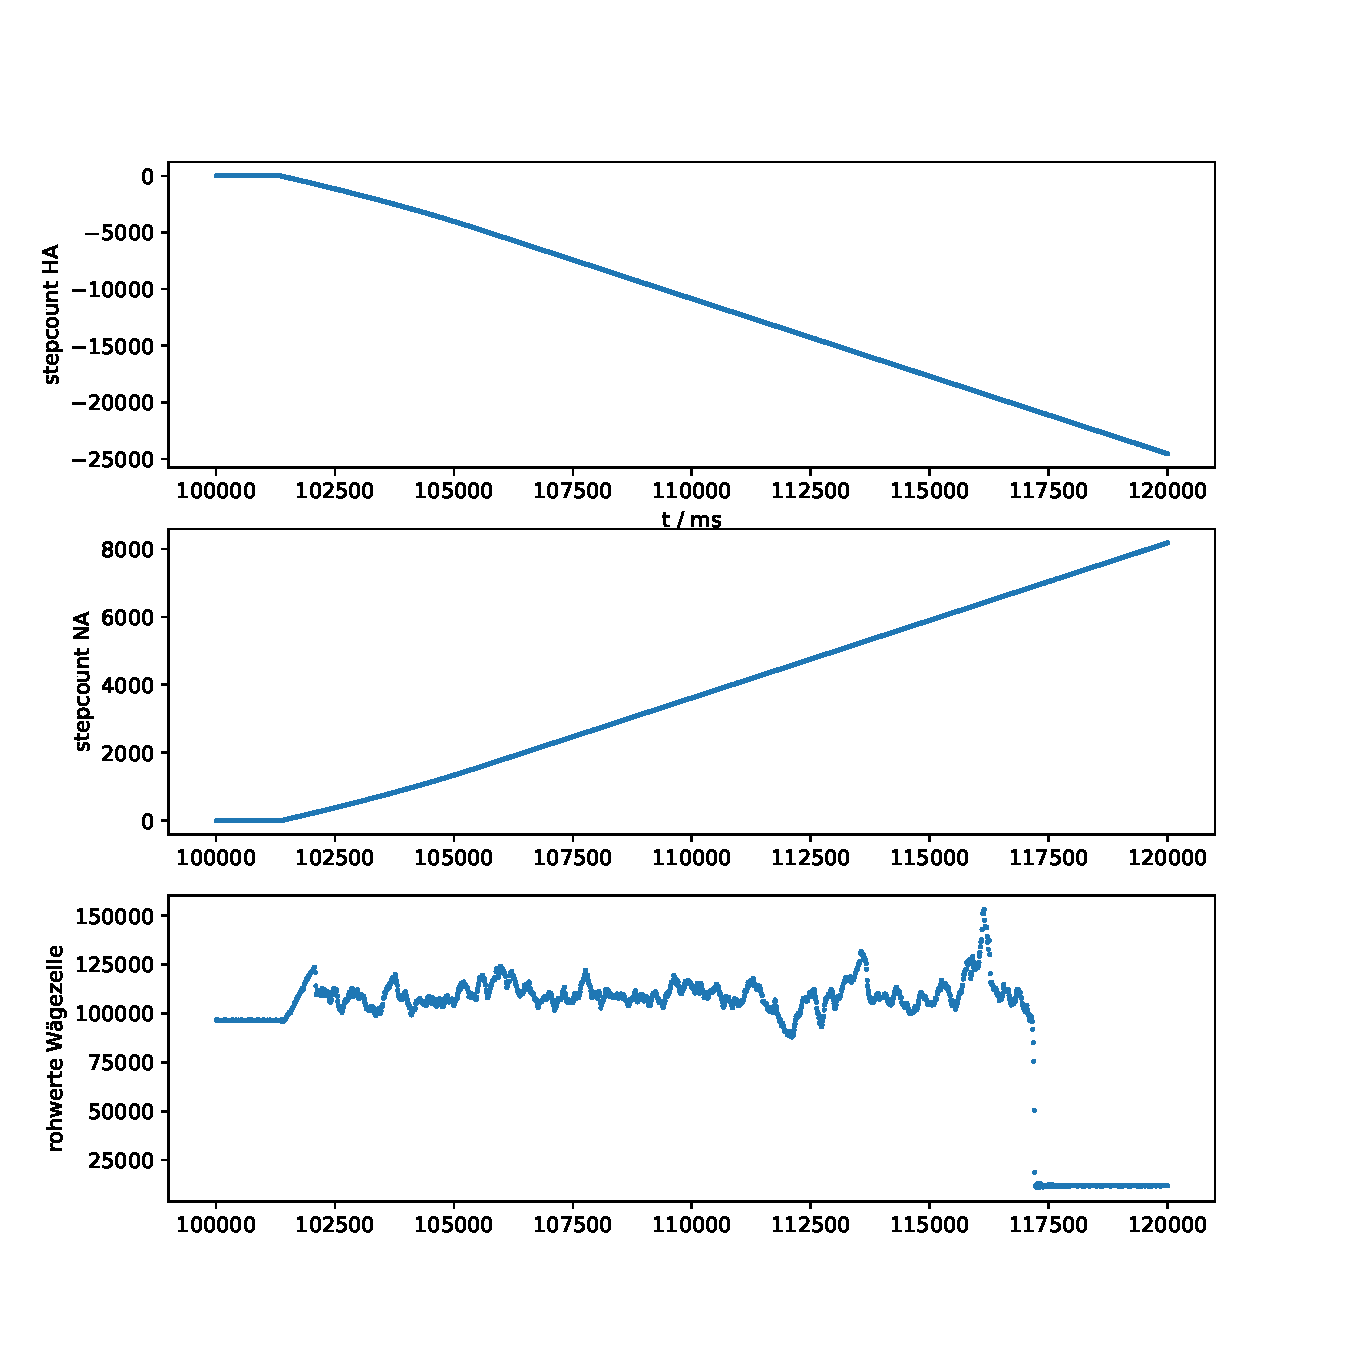
\includegraphics[width=0.9\textwidth]{./roh.pdf}
    \caption{Rohdaten einer Messung mit Fadenabriss. Die X-Achse beschreibt in allen drei Grafiken die Zeit $t$.}
    \label{fig:rohdaten_abriss}
\end{figure}